\section{Real-Life Use Cases}
\label{sec:usecases}

The five conditions in \S\ref{sec:fair} identify a narrow niche. Here we
name concrete workloads that satisfy them, each grounded in a measured
result in this repo.

\subsection{Serial investigation chains}

A security operations centre receives an alert, looks up threat
intelligence, cross-references internal logs, generates a hypothesis, and
drills into the next layer. Each hop blocks on the previous one;
concurrency is 1 by construction. This is the workflow for SOC analysts,
forensic investigators, and multi-hop debugging pipelines.

We measured chain depths $D \in \{1,3,5,10,20\}$ on both arms
(\artifact{results/chain\_analysis.json},
\artifact{results/chain\_\{ar3b,dg\}.json}, BGL, $n{=}300$). Both models are
linear in depth (slope CV 1.1\% for DG, 1.2\% for AR). DG's per-hop p50 is
$\sim$410\,ms against AR's $\sim$825\,ms --- a $2.0\times$ advantage that is
constant across depth. DG's tail penalty (the 3.21$\times$ max/median from
Appendix~\ref{app:distributions}) washes out under sequential composition:
the p99.9/median ratio converges from 1.04$\times$ at $D{=}1$ to
1.77--2.07$\times$ at $D{=}10$--$20$, against AR's 1.93$\times$ mean.

\begin{figure}[t]
\centering
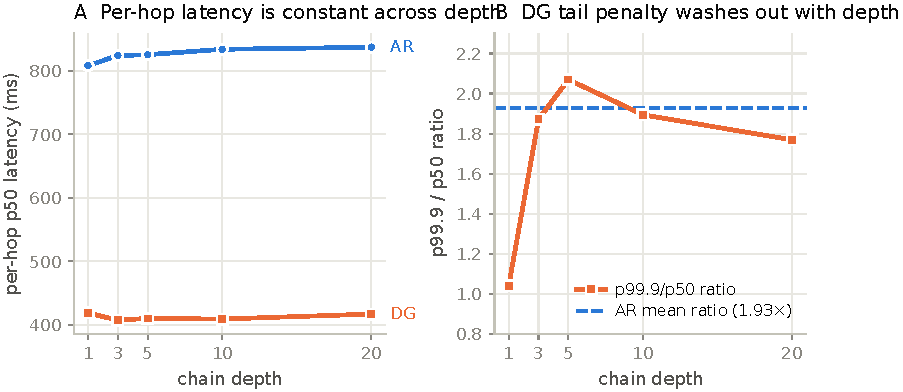
\includegraphics[width=\linewidth]{figures/fig10_usecase_chains.pdf}
\caption{Serial investigation chains
(\artifact{results/chain\_analysis.json}, BGL, $n{=}300$). \textbf{A:}
per-hop p50 is constant across depth for both models; DG is $2.0\times$
faster. \textbf{B:} DG's p99.9/p50 ratio (high in isolation) converges to
AR's mean as depth increases --- the tail penalty washes out under
sequential composition.}
\label{fig:chains}
\end{figure}

The batching multiplier that makes AR dominant in aggregate throughput is
unavailable here by construction. The serial-vs-serial comparison is the
operative one, and DG leads it.

\subsection{Critical-alert preemption}

A FATAL log line arrives mid-stream while batch work is in flight. The
structured record must be fresh within 1\,s. Trading dashboards,
safety-critical monitoring, alarm triage, and on-call paging all have this
shape: most work is background, but one request is urgent.

We measured vLLM 0.25.1's preemption policies on both arms
(\artifact{results/vip\_\{ar3b,dg\}.json}, BGL). DG's lower service time
($\sim$420\,ms vs AR's $\sim$660--800\,ms at task lengths) is available on
demand via per-request priority preemption, and it survives the
\texttt{max-num-seqs 1} constraint that the mixed-phase crash forces.
AR's batching advantage is irrelevant for the one request that matters.

\subsection{Autonomous driving and safety-critical perception}

An autonomous vehicle perceives a hazardous scene --- a pedestrian entering
a blind crosswalk, debris on a highway, a construction zone with temporary
lane closures --- and must produce a structured situation report and action
plan before the next control tick. The output is long (multi-object scene
description, predicted trajectories, recommended manoeuvre), the latency
budget is sub-second, and the system is strictly batch-1: there is one
vehicle, one scene, one decision. There is no queue to batch against.

DG's properties map directly onto this workload. The staircase cost law
means the p50 is flat whether the scene report is 128 or 512 tokens ---
the model does not pay per token the way an autoregressive decoder does.
The $K$ knob (Appendix~\ref{app:decomp}) is a per-request quality slider:
drop $K$ from 8 to 4 and the record arrives in \kFourPfifty\,ms at
\kFourFone\ F1, meeting a tightened deadline without truncating the output.
An AR model under the same deadline returns a truncated record that fails
schema validation --- a partial scene description is not a partial plan, it
is a failed plan. The diffusion model always returns a complete canvas,
which for a safety-critical consumer that validates against a schema is a
qualitative rather than quantitative guarantee --- \emph{provided the output
length budget is sufficient}. Below the natural record length the diffusion
model's schema validity collapses (1.0\% at $L{=}128$, see
Appendix~\ref{app:quality}); the completeness guarantee holds only at or
above the canvas length where the model was calibrated.

The tail latency (Appendix~\ref{app:distributions}) is the counterargument:
DG's 3.21$\times$ max/median ratio means a p99 SLA lands far above p50. For
autonomous driving this is managed by the $K$ knob (lower $K$ compresses
the tail) and by the serial-chain result (consecutive hops wash out the
tail). A single-hop, hard-deadline perception task is the regime where DG
is weakest, and we state that plainly.

\subsection{Algorithmic trading and multi-hop situation analysis}

A trading system detects an anomalous price movement, pulls relevant
order-book history, cross-references news and regulatory filings, and
produces a structured hypothesis: is this a mean-reversion signal, a
liquidity event, or a precursor to a larger move? Each step blocks on the
previous one --- the analysis is a chain, not a batch. The output at each
hop is a structured record (event classification, confidence, recommended
action), and the total latency from signal to decision must be under the
market's reaction window, typically 1--5 seconds.

This is the serial investigation chain of \S\ref{sec:usecases} applied to
market microstructure. DG's per-hop latency of $\sim$410\,ms (measured,
Figure~\ref{fig:chains}) means a 5-hop analysis completes in
$\sim$2.1\,s; AR's $\sim$825\,ms per hop gives $\sim$4.1\,s for the same
chain. At 10 hops the gap is 4.1\,s vs 8.3\,s --- the difference between
acting before and after the market moves. The tail penalty that makes DG
risky in single-hop, hard-deadline settings washes out under sequential
composition: the p99.9/p50 ratio converges to the AR mean at depth 10+.

The quality-comparable AR model (1.5B, \arOneFiveFnine\ F1) is $1.8\times$
slower per hop even unforced. In a market where the first analysis wins,
that margin is the trade.

\subsection{Long structured extraction}

Java stack traces, Kubernetes event cascades, and correlated alert bursts
produce output that naturally exceeds 256 tokens. At forced $L{=}512$
(\artifact{results/appD\_mult\_\{ar3b,dg\}\_L512.json}, BGL, $n{=}300$):

\begin{center}
\begin{tabular}{@{}lrrl@{}}
\toprule
 & AR-3B & DG & \\
\midrule
p50 (ms)    & 3223 & 524  & DG $6.2\times$ faster \\
9-field F1  & 0.852 & 0.855 & comparable \\
\bottomrule
\end{tabular}
\end{center}

AR forced to emit 512 tokens when the record needs $\sim$150 rambles and
corrupts even structural copy-from-input fields. DG's canvas fills the
record plus padding without degrading --- masked diffusion is
length-robust where autoregression is not. At long output this is a
qualitative advantage, not just a speedup.

\subsection{Wide-schema normalisation}

Financial transaction records, complex telemetry, and compliance reports
can carry 50--100 fields with pairwise consistency constraints that grow
as $O(F^2)$. We measured schema widths $F \in \{12, 25, 50, 100\}$
(\artifact{results/wide\_schema\_\{ar3b,dg\}.json}, BGL). DG's latency
advantage holds at $1.8$--$3.0\times$ across widths. Consistency drops
from 91\% to 87\% at 50 fields but plateaus --- the joint-canvas
denoising (all fields denoised together) absorbs the structural coherence
cost. AR generates fields one at a time with no mechanism to enforce
inter-field constraints except through the prompt.

\begin{figure}[t]
\centering
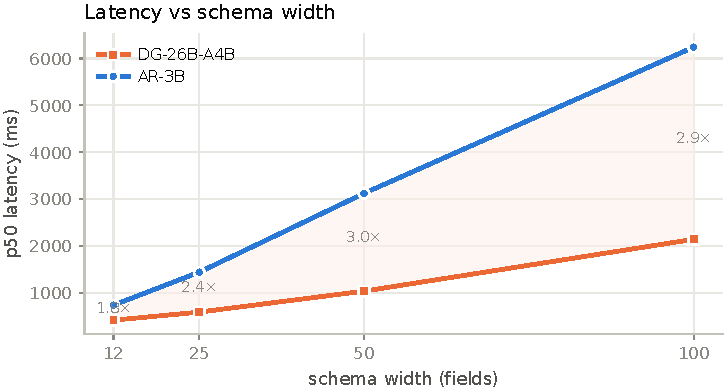
\includegraphics[width=0.85\linewidth]{figures/fig11_usecase_schema.pdf}
\caption{Latency vs schema width
(\artifact{results/wide\_schema\_\{ar3b,dg\}.json}, BGL, $n{=}300$). The
gap widens with field count: AR's left-to-right generation pays per field,
while DG's joint denoising treats all fields as one structured object.}
\label{fig:schema}
\end{figure}

\subsection{Edge and single-tenant deployments}

Industrial controllers, network probes, IoT gateways, and regulated
environments (HIPAA, SOC2) where cross-request batching is disallowed.
At $B{=}1$ the entire throughput case for AR collapses: the serial-vs-serial
number is the operative one, and DG leads it. DG's cost-invariance to
output size also means the p99 is flat whether the record is 128 or 512
tokens, where AR's p99 grows linearly.

\subsection{Where diffusion does not win}

The boundary is sharp. High-rate log streams ($\lambda \gg
\crossoverLambda$ ev/s) favour AR's batching by 50--80$\times$. Tail-sensitive
single-stream workloads with strict p99 SLAs are hurt by DG's 3.21$\times$
max/median ratio (though this washes out under sequential composition, as
the chain experiment shows). And any workload that can batch favours AR
regardless of output length.
